% Werke X/1 (1917), native145–149, printed138–142.
\SourceLeaf{145}\NoSourceHead
\HistoricTitle{NACHLASS.}
\pdfbookmark[1]{Exercitationes mathematicae}{exercitationes}
\HistoricTitle{EXERCITATIONES MATHEMATICAE.}
\HistoricCitation{[Zettel in Fh, Kapsel 50.]}
\NumberedItem{1}
\begin{center}\itshape Demonstratio elementaris propositionis de productis e Cosinibus.\end{center}
\[\begin{aligned}
\sin\tfrac1{13}\pi\mathpunct{.}\cos\tfrac1{13}\pi&=\tfrac12\sin\tfrac2{13}\pi\\
\tfrac12\sin\tfrac2{13}\pi\mathpunct{.}\cos\tfrac2{13}\pi&=\tfrac14\sin\tfrac4{13}\pi
\end{aligned}\]
\noindent\& sic porro et si tandem
\[\sin\frac{2^n\pi}{13}=\pm\sin\frac1{13}\pi\]
\noindent erit
\[\frac1{2^n}=\pm\cos\frac1{13}\pi\mathpunct{.}\cos\frac2{13}\pi\mathpunct{.}\cos\frac4{13}\pi\ldots\cos\frac{2^{n-1}}{13}\pi.\]
\noindent Eodem modo demonstratur productum
\[\cos\frac m{13}\pi\mathpunct{.}\cos\frac{2m}{13}\pi\ldots\cos\frac{2^{n-1}m}{13}\pi\]
\noindent dare idem productum. Hae veritates etiam aeque facile absque omni calculo
per solam polygoni inspectionem demonstrantur.
\par\noindent\hfill\textit{Aug. 21. 96.}\par
\ClosingRule
\clearpage
\SourceLeaf{146}\ArithmeticHead{139}{R}{EXERCITATIONES MATHEMATICAE.}
\NumberedItem{2}
\noindent\hspace*{\parindent}Perfacilis est demonstratio geometrica propositionis
\[\cos0+\cos\tfrac{2\pi}n+\cos\tfrac{4\pi}n+\cos3\tfrac{2\pi}n+\ldots+\cos(n-1)\tfrac{2\pi}n\ \text{esse}=0,\]
\noindent si polygonum in hoc situ consideretur:
\begin{center}
\begin{tikzpicture}[x=.006cm,y=-.006cm,line width=.55pt]
\draw[dash pattern=on 2.3pt off 3.2pt] (25,452)--(1228,452);
\draw[dash pattern=on 2.3pt off 3.2pt] (270,38)--(270,457);
\draw[dash pattern=on 2.3pt off 3.2pt] (318,296)--(318,457);
\draw[dash pattern=on 2.3pt off 3.2pt] (971,294)--(971,454);
\draw[dash pattern=on 2.3pt off 3.2pt] (1015,33)--(1015,454);
\draw (275,36)--(318,296)--(519,457)--(777,457)--(971,294)--(1014,33);
\end{tikzpicture}
\end{center}
\noindent\hfill\textit{Eodem.}\par
\ClosingRule
\NumberedItem{3}
\noindent\hspace*{\parindent}Summa Serierum periodos quarum summa $=0$ tenentium commode invenitur,
si singula membra per successivas variabilis cuiusdam $x$ potestates
multiplicentur, unde huius seriei, quae est recurrens, summa sic exhibetur:
\[\frac{a+bx+cxx+\ldots}{1-x^n},\]
\noindent quae pro nostro casu $x=1$ abit in hanc formam $\frac00$. Si valor huius expressionis
per regulas notas investigetur, ad eadem pervenietur, quae B[eatus]
D[\textsc{aniel}] \textsc{Bern[oulli]} ex principio metaphysico, sc. rationis sufficientis eruerat.
\par\noindent\hfill\textit{Aug. 28. 96.}\par
\ClosingRule
\vfill\noindent\hfill18\textsuperscript{*}\hspace*{.12\linewidth}\par
\clearpage
\SourceLeaf{147}\ArithmeticHead{140}{L}{ANALYSIS.\quad NACHLASS.}
\NumberedItem{4}
\[\text{Lim. }\frac{\Sigma\,\text{pr. ad }n\text{ infra }n}{nn}\]
\noindent (Pr. usque ad $P+30n$) sunt
\[(4-1)(3^2-1)(5^2-1)n=576n\]
\noindent ideo a
\[P\ldots Pn\quad\text{generaliter}\quad
\frac{1\mathpunct{.}3}{2\mathpunct{.}2}\mathpunct{.}\frac{2\mathpunct{.}4}{3\mathpunct{.}3}\mathpunct{.}\frac{4\mathpunct{.}6}{5\mathpunct{.}5}\ldots nn.\]
\noindent Si $P:n=\infty:1$
\par\noindent adeoque
\[\begin{aligned}
\text{Limes quaesitus}&=\tfrac12\mathpunct{.}\frac{1\mathpunct{.}3}{2\mathpunct{.}2}\mathpunct{.}\frac{2\mathpunct{.}4}{3\mathpunct{.}3}\mathpunct{.}\frac{4\mathpunct{.}6}{5\mathpunct{.}5}\ldots\\
&=\frac3{\pi\pi}=\frac3{9{,}8696}=0{,}3039+
\end{aligned}\]
\ClosingRule
\NumberedItem{5}
\noindent\hspace*{\parindent}Si $\Phi$ significet eiusmodi functionem ut sit
\[\Phi:\int\frac{dx}{\surd(1-x^3)}=x,\]
\noindent erit
\[\begin{aligned}
\Phi x={}&x-\tfrac12\mathpunct{.}\tfrac14Ax^3+\tfrac36\mathpunct{.}\tfrac17Bx^3-\tfrac58\mathpunct{.}\tfrac1{10}Cx^3\\
&+\tfrac1{13}\mathpunct{.}\tfrac9{12}Dx^3-\tfrac1{16}\mathpunct{.}\tfrac{11}{14}Ex^3
(+\tfrac1{19}\mathpunct{.}\tfrac{15}{18}Fx^3-\tfrac1{22}\mathpunct{.}\tfrac{17}{21}Gx^3+\ldots)
\end{aligned}\]
\noindent Seu concinnius
\[\begin{aligned}
={}&x-\frac{1\mathpunct{.}3}{2\mathpunct{.}3\mathpunct{.}4}Ax^3
+\frac{3\mathpunct{.}5}{5\mathpunct{.}6\mathpunct{.}7}Bx^3
-\frac{5\mathpunct{.}9}{8\mathpunct{.}9\mathpunct{.}10}Cx^3\\
&+\frac{9\mathpunct{.}11}{11\mathpunct{.}12\mathpunct{.}13}Dx^3
-\frac{11\mathpunct{.}15}{14\mathpunct{.}15\mathpunct{.}16}Ex^3+\ldots
\end{aligned}\]
\ClosingRule
\clearpage
\SourceLeaf{148}\ArithmeticHead{141}{R}{EXERCITATIONES MATHEMATICAE.}
\NumberedItem{6}
\noindent\hspace*{\parindent}Si
\[\Phi:\int\frac{dx}{\surd(1-x^4)}=x,\]
\noindent erit
\[\Phi x=x-\frac1{10}x^5+\frac1{120}x^9-\frac{11}{15600}x^{13}+\frac{211}{13000\mathpunct{.}272}x^{17}-\ldots\]
\begin{center}.\quad .\quad .\quad .\quad .\quad .\quad .\quad .\quad .\quad .\quad .\quad .\quad .\quad .\quad .\quad .\quad .\quad .\end{center}
\ClosingRule
\NumberedItem{7}
\noindent\hspace*{\parindent}Incumbant corpora $A,B,C$ \&c plano hor[izontali] (quod sine frictione
concipimus) filis utcunque connexa; applicetur filo in $E$ potentia secundum
$EF$, ita ut punctum $E$ semper super hac linea protrahatur; quaeritur motus
corporum $A,B,C,\ldots$
\begin{center}
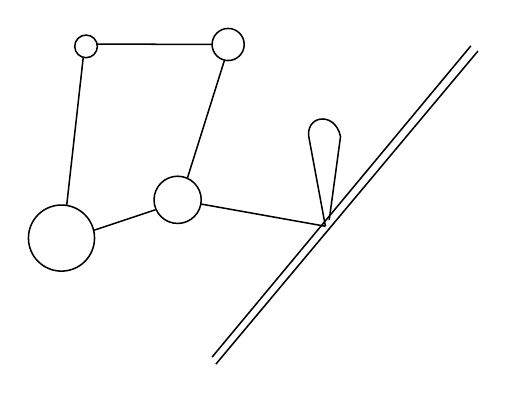
\begin{tikzpicture}[x=.006cm,y=-.006cm,line width=.55pt]
\draw (163,89) circle[radius=24];
\draw (464,85) circle[radius=34];
\draw (111,495) circle[radius=70];
\draw (357,414) circle[radius=50];
\draw (185,84)--(430,85);
\draw (157,113)--(122,426);
\draw (456,119)--(378,367);
\draw (178,479)--(310,435);
\draw (407,423)--(670,470);
\draw (670,470)--(636,287) .. controls (623,235) and (690,224) .. (702,280)--(678,457);
\draw (430,747)--(978,88);
\draw (438,762)--(993,99);
\end{tikzpicture}
\end{center}
\ClosingRule
\NumberedItem{8}
\noindent\hspace*{\parindent}Investigare polyhedra regularia, quae originem ducunt a polygonis huius
figurae
\clearpage
\SourceLeaf{149}\ArithmeticHead{142}{L}{ANALYSIS.\quad NACHLASS.}
\begin{center}
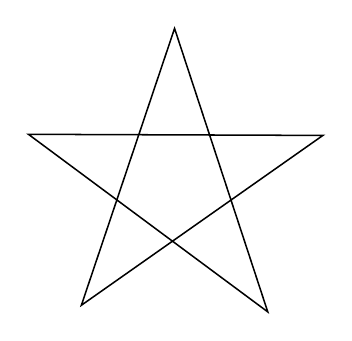
\begin{tikzpicture}[x=.007cm,y=-.007cm,line width=.55pt]
\draw (301,28)--(470,542)--(36,220)--(570,222)--(132,530)--cycle;
\end{tikzpicture}
\end{center}
\noindent Quot formas diversas polyg[onum] hab[ere] potest?
\[\text{Resp[onsio]: }\frac{\text{Num: primorum infra }N\text{ ad }N}{2}\]
\begin{center}.\quad .\quad .\quad .\quad .\quad .\quad .\quad .\quad .\quad .\quad .\quad .\quad .\end{center}
\ClosingRule
\NumberedItem{9}
\noindent\hspace*{\parindent}Evolvere prod[ucta]
\[\begin{gathered}
1-x\mathpunct{.}1-x^2\mathpunct{.}1-x^3\mathpunct{.}1-x^4\ldots\\
1-x\mathpunct{.}1-x^2\mathpunct{.}1-x^4\ldots
\end{gathered}\]
\ClosingRule
\NumberedItem{10}
\noindent\hspace*{\parindent}Invenire
\[\text{Lim: }\frac{\Sigma\,\text{pr. ad }n\text{ infra }n}{nn}\]
\[\pm\quad0{,}307.\]
\ClosingRule
\NumberedItem{11}
\noindent\hspace*{\parindent}Ex aeq[uationibus]
\[\begin{array}{r|r|r|r}
0=Aa'&=Aa''&=Aa'''&=Aa^{\mathrm{IV}}\\
+Ba''&+Ba'''&+Ba^{\mathrm{IV}}&+Ba'\\
+Ca'''&+Ca^{\mathrm{IV}}&+Ca'&+Ca''\\
+Da^{\mathrm{IV}}&+Da'&+Da''&+Da'''
\end{array}\]
\clearpage
